%Siehe tolle Daten in Tab. \ref{tab:impl:data}.
%
%\begin{table}
%    \centering
%    \begin{tabular}{|lcc|}
%    \hline
%              & \textbf{Regular Customers} & \textbf{Random Customers} \\ \hline
%    Age       & 20-40                      & \textgreater{}60          \\ \hline
%    Education & university                 & high school               \\ \hline
%    \end{tabular}
%    \caption{Ein paar tabellarische Daten}
%    \label{tab:impl:data}
%\end{table}
%
%\begin{figure}
%    \centering
%    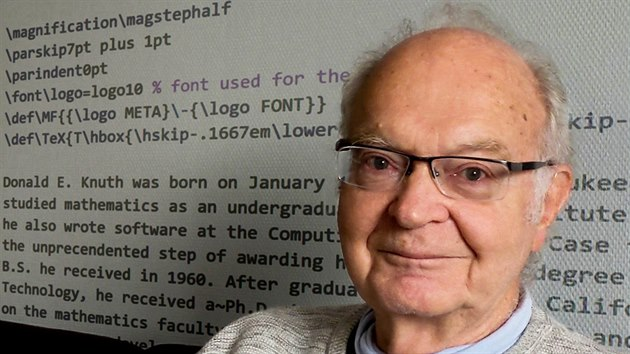
\includegraphics[scale=0.5]{pics/knuthi.jpg}
%    \caption{Don Knuth -- CS Allfather}
%    \label{fig:impl:knuth}
%\end{figure}
%
%Siehe und staune in Abb. \ref{fig:impl:knuth}.
%\lipsum[6-9]
%Dann betrachte den Code in Listing \ref{lst:impl:foo}.
%
%\begin{lstlisting}[language=Python,caption=Some code,label=lst:impl:foo]
%# Program to find the sum of all numbers stored in a list (the not-Pythonic-way)
%
%# List of numbers
%numbers = [6, 5, 3, 8, 4, 2, 5, 4, 11]
%
%# variable to store the sum
%sum = 0
%
%# iterate over the list
%for val in numbers:
%    sum = sum+val
%
%print("The sum is", sum)
%\end{lstlisting}



\section{Mobile App}
\setauthor{Dominik Ortbauer}

The mobile app was developed with react-native and Expo. 
The setup for both was very simple and finished after a few npm commands.

The app consists of multiple screens which are all accessible from the bottom tab-bar:
One screen for taking pictures of the application form\ref{fig:impl:camscreen}, a second one to view the images\ref{fig:impl:galleryscreen}, a third one used for validating the data returned from the model\ref{fig:impl:validationscreen} and a fourth and final one to access the settings\ref{fig:impl:settingsscreen}.

\subsection{Camera Screen}

The camera screen features a view of the cameras view,
a small thumbnail for the last taken picture which leads you to the gallery screen when pressed,
a button to take a picture and a button to to send the pictures to the model.
It is impotent to notice that the pictures are NOT saved on the users phone.

The structure for the CameraScreen consists of one view containing the camera, another view for the thumbnail and take photo button as well as the button for sending the pictures to the backend. This view stacks them vertically on top of one another and the view for the thumbnail and picture button orders them horizontally.

\begin{lstlisting}[caption=CameraScreen display code,label=lst:impl:cameraScreenDisplay]
<View style={styles.container}>
  <Camera
    style={styles.camera}
    type={CameraType.back}
    ref={ref => setCameraRef(ref)}
  />
  <View style={styles.horizontalContainer}>
    {
      state.pictures.length > 0 ?
      <View style={styles.thumbnailContainer}>
        <TouchableOpacity onPress={() => navigation.navigate('Gallery')}>
          <Image style={styles.thumbnail} source={state.pictures[0]}></Image>
        </TouchableOpacity>
      </View>
      :
      <View></View>
    }
    
    <TouchableOpacity style={styles.button} onPress={takePicture}>
      <Text style={styles.buttonText}>Photo</Text>
    </TouchableOpacity>
  </View>
  
  <TouchableOpacity style={styles.button} onPress={sendToProcessing}>
    <Text style={styles.buttonText}>Abschicken</Text>
  </TouchableOpacity>
</View>
\end{lstlisting}

The CameraScreen\ref{fig:impl:camscreen} asks for permissions to access the camera if it does not already have them.

\begin{lstlisting}[caption=Code for camera permissions,label=lst:impl:campermissions]
React.useEffect(() => {
    (async () => {
        const { status } = await requestCameraPermissionsAsync();
        setHasPermission(status === 'granted');
    })();
}, []);
\end{lstlisting}

Whenever the picture trigger is pressed the below code which makes the camera take a picture and append it to the start of the pictures list will be executed. 

\begin{lstlisting}[caption=Code for taking pictures,label=lst:impl:takepicture]
const takePicture = async () => {
    if (cameraRef) {
        const photo = await cameraRef.takePictureAsync();
    
        dispatch({pictures: [photo, ...state.pictures]});
    }
};
\end{lstlisting}

\subsection{Gallery Screen}

If there are not any pictures taken the gallery screen just displays ``no pictures taken'' but if pictures where taken beforehand
it displays the pictures newest first and allows you to switch between the pictures with arrows(right to go to older pictures and left to go to newer ones)
the left arrow does not display while the newest picture is active and the right arrow does not display while the oldest one is active.
There is button for deleting a picture and one for replacing one which just deletes the picture and takes you to the camera screen.

The Gallery Screen has a view which contains the image, the left/right arrows and the toolbar.
The arrows use absolute positioning to appear right and left respectively.
The delete and replace buttons are both inside a View which is positioned absolute at the bottom of the screen and they are ordered as a row.


\begin{lstlisting}[caption=Gallary Screen display code,label=lst:impl:galleryScreenDisplay]
<View style={styles.container}>
    {
        state.pictures.length > 0 ? 
        <ImageBackground resizeMode="contain" style={styles.image} source={state.pictures[index]}></ImageBackground> 
        :
        <Text>No Pictures taken</Text>
    }
    {
        index > 0 ? 
        <TouchableOpacity style={styles.navigationLeft} onPress={() => setIndex(index - 1)}>
        <MaterialIcons name='arrow-left' color={'#1976D2'} size={70} />
        </TouchableOpacity>
        :
        <View></View>
    }
    {
        index < state.pictures.length - 1 ?
        <TouchableOpacity style={styles.navigationRigth} onPress={() => setIndex(index + 1)}>
        <MaterialIcons name='arrow-right' color={'#1976D2'} size={70} />
        </TouchableOpacity>
        :
        <View></View>
    }
    {
        state.pictures.length > 0 ?
        <View style={styles.toolbarContainer}>
            <TouchableOpacity onPress={() => removePicture()}>
                <MaterialIcons name='delete' color={'#1976D2'} size={50}/>
            </TouchableOpacity>
            <TouchableOpacity onPress={() => {removePicture(); navigation.navigate('Camera')}}>
                <MaterialIcons name='edit' color={'#1976D2'} size={50}/>
            </TouchableOpacity>
        </View>
        :
        <View></View>
    }
</View>
\end{lstlisting}

\subsection{Validation Screen}

The validation screen displays the data returned from the model with the values from the application form.
The data sent between the client and the server is always an applicant, as shown in the below listing, as a json. First the server sends the not yet validated applicant to the client which then sends the validated applicant back.
For each field of the applicant the validation screen displays a Label and depending on the datatype either a Textbox, a Textbox which only allows numbers or a checkbox for boolean fields.
After the validation is done the validated data can be sent back to  the server which then enters it into the access database.


\begin{lstlisting}[language=typescript,caption=Classes for applicant(Bewerber) and legal guardian(Erziehungsberechtigter),label=lst:impl:applicantGuardian]
export class Bewerber {
    nachname: string;
    vornamen: string;
    wunsch_abteilung: string;
    alternativ_abteilung: string;
    alternativ_abteilung2: string;
    geschlecht: string;
    svn_kurz: number;
    geburtsdatum: string;
    telefonnummer: string;
    vorschule_jahre: string;
    volkschule_jahre: string;
    mittelschule_jahre: string;
    ahs_jahre: string;
    poly_jahre: string;
    sonstige_jahre: string;
    herkunftsschule_typ: string;
    herkunftsschule_name: string;
    geburtsstaat: string;
    staatsbuergerschaft: string;
    muttersprache: string;
    alltagssprache: string;
    religion: string;
    schulpflicht_erfuellt: boolean;
    geschwister_an_der_schule: boolean;
    verhalten7sst: string;
    original_jahreszeugnis: boolean;
    erziehungsberechtigte: Erziehungsberechtigter[];
}

export class Erziehungsberechtigter {
    type: string;
    anrede: string;
    title: string;
    akad_grad: string;
    vorname: string;
    zweiter_vorname: string;
    nachname: string;
    akad_grad_nach: string;
    land: string;
    plz: string;
    gemeinde: string;
    strasse: string;
    hausnummer: string;
    telefonnummer1: string;
    telefonnummer2: string;
    email: string;
    schueler_wohnt_hier: boolean;
    ist_erziehungsberechtigt: boolean;
}
\end{lstlisting}

\begin{lstlisting}[language=typescript,caption=Code to display one field,label=lst:impl:field]
<View key={field} style={styles.container}>
  <Text style={styles.label}>{field}:</Text>
  {typeof studentData[field] === "boolean" ? (
    <CheckBox
      checked={studentData[field]}
      onPress={() =>
        handleStudentDataChange(field, !studentData[field])
      }
    />
  ) : (
    <View />
  )}
  {typeof studentData[field] === "string" ? (
    <TextInput
      style={styles.input}
      value={studentData[field]}
      onChangeText={(text) => handleStudentDataChange(field, text)}
    />
  ) : (
    <View />
  )}
  {typeof studentData[field] === "number" ? (
    <TextInput
      style={styles.input}
      value={
        studentData[field].toString() == "NaN"
          ? ""
          : studentData[field].toString()
      }
      onChangeText={(text) => handleStudentDataChange(field, text)}
    />
  ) : (
    <View />
  )}
</View>
\end{lstlisting}

\FloatBarrier

\begin{figure}
    \centering
    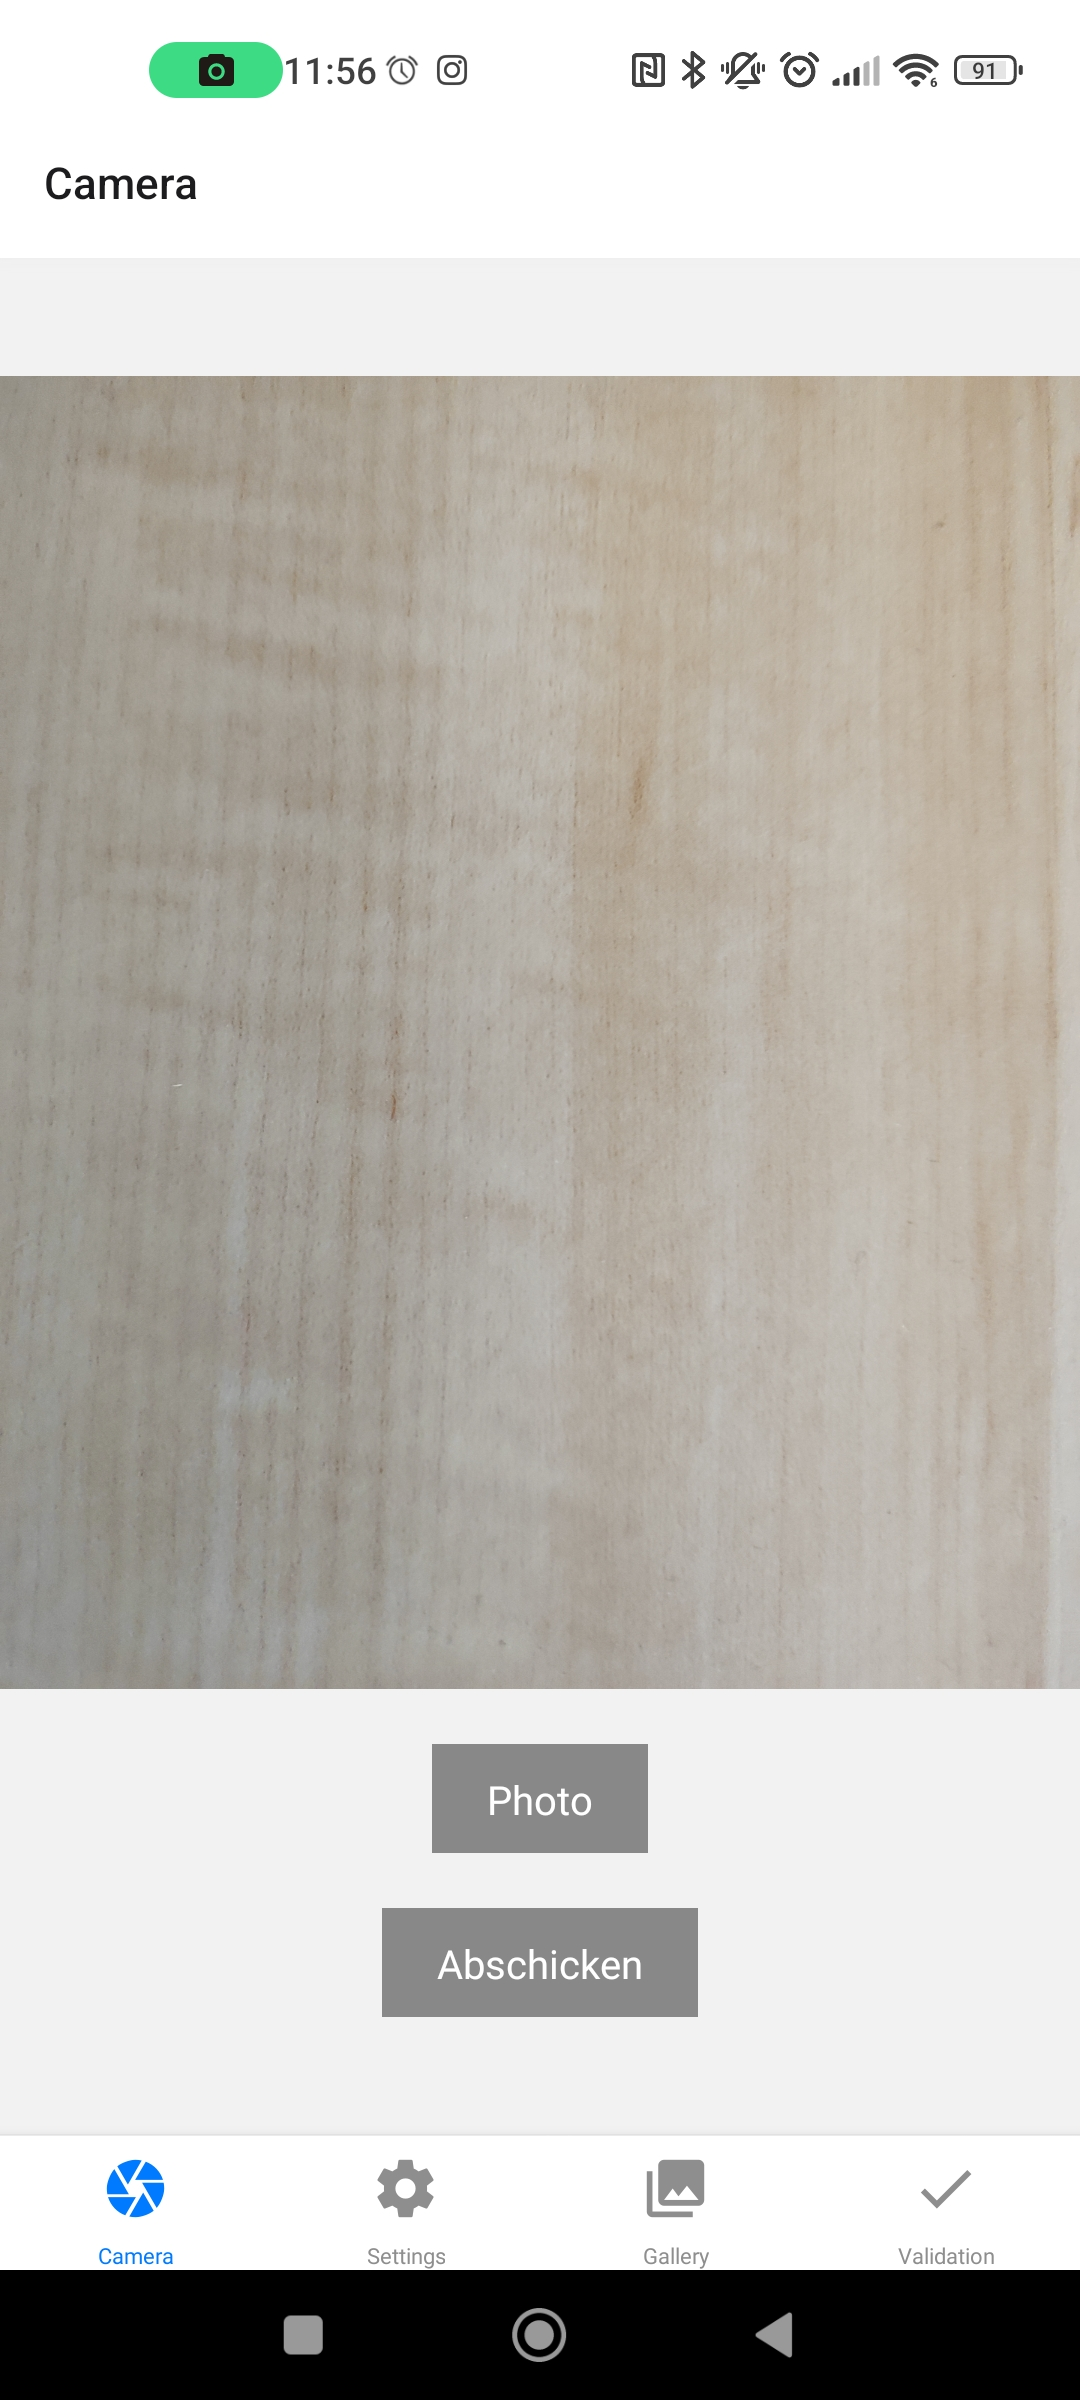
\includegraphics[scale=0.2]{pics/CameraScreen.jpg}
    \caption{Camera Screen}
    \label{fig:impl:camscreen}
\end{figure}

\begin{figure}
    \centering
    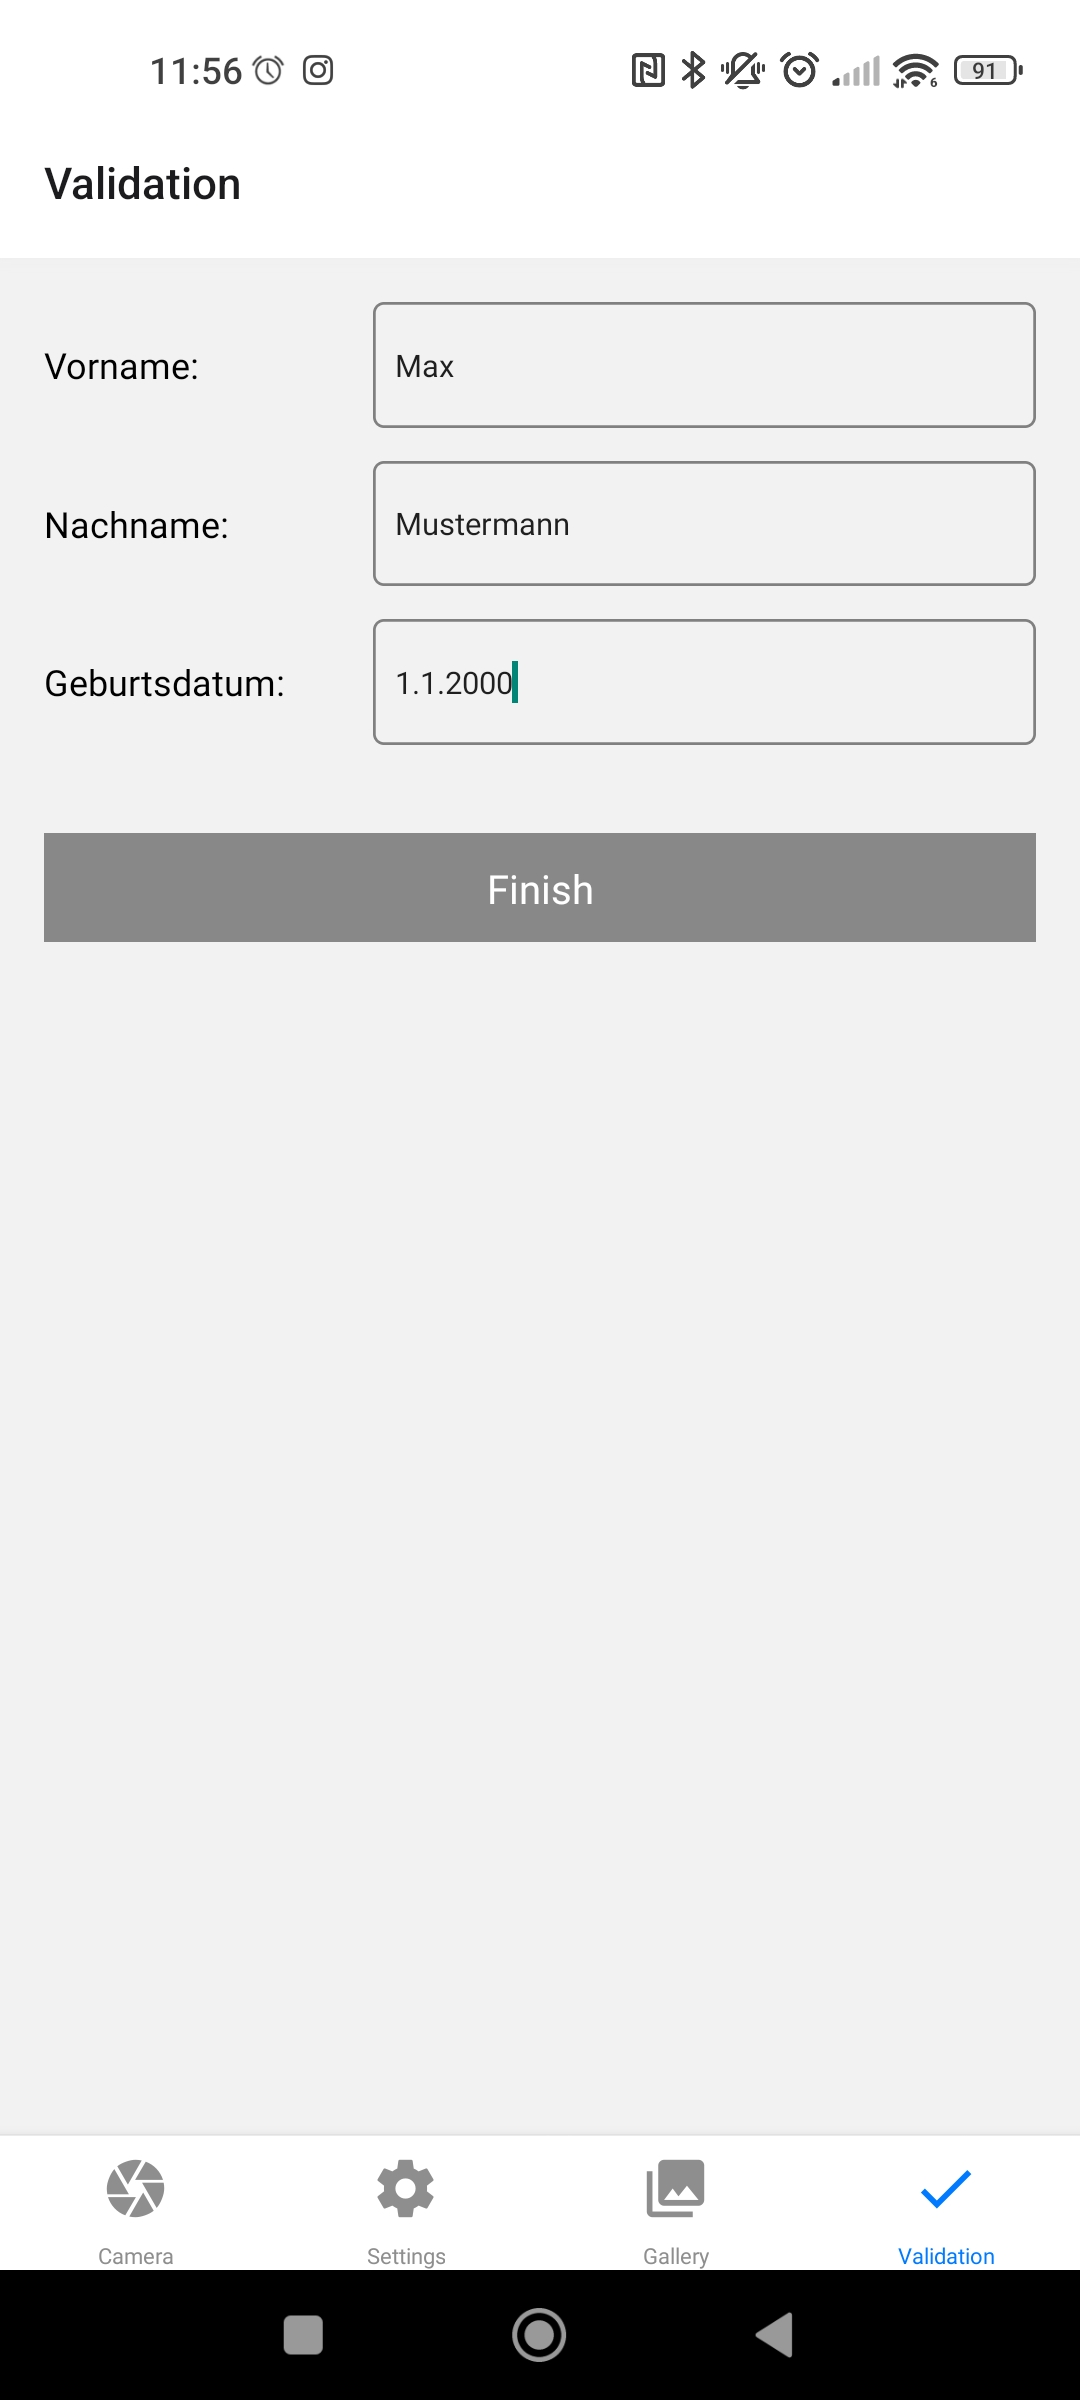
\includegraphics[scale=0.2]{pics/ValidationScreen.jpg}
    \caption{Validation Screen}
    \label{fig:impl:validationscreen}
\end{figure}

\FloatBarrier

\subsection{SocketClient}

The communication with the backend is handled inside the SocketClient class which takes care of establishing a connection to the model as well as sending and receiving data.
A SocketClient is created when you start the app or when changing the settings for connecting to the backend. The host and port are stored in an AsyncStorage.

The following code shows the constructor for the SocketClient class.
When creating a SocketClient it needs a host and port to identify where to connect to. These two values can be set in the settings screen\ref{fig:impl:settingsscreen}.
The onMessage callback is important for receiving messages because it will be called every time a message is received and get the data from the message passed along.

Whenever an error occurs with the connection one second is waited and then a new connection will be established.

\begin{lstlisting}[caption=Constructor for the SocketClient,label=lst:impl:constructorSocketClient]
constructor(host: string, port: number, onMessage: (data: any) => void) {
    this.port = port;
    this.host = host;
    this.onMessage = onMessage;
    this.ws = this.createWebSocket();
}

private createWebSocket(): WebSocket {
    const ws: WebSocket = new WebSocket(`ws://${this.host}:${this.port}`);

    ws.onerror = (error) => {
        console.log(`WebSocket error: ${error.message}`);

        async function sleep(ms: number) {
            return new Promise(resolve => setTimeout(resolve, ms));
        }

        (async() => {
            await sleep(1000);
            this.ws = this.createWebSocket();
        })();
        
        ws.close();
    }

    ws.onopen = () => {
        console.log("Connected to server");
    };

    ws.onmessage = (json) => {
        const data = JSON.parse(json.data);
        console.log(data)
        this.onMessage(data);
    };

    return ws;
}
\end{lstlisting}

For sending images to the model the sendProcessingData method is used.
The method takes a CameraCapturedPicture Array which will be read and sent to the websocket backend.
The content of the image is not immediately present in a CameraCapturedPicture but has to be read from the URL property of it.
The following code reads the content of all the pictures using a FileReader and creates a json from it containing the base64 encoded content of each picture.

The type property of the json being sent is used by the backend to determine the difference between receiving pictures and receiving the validated data.



\begin{lstlisting}[caption=Method for sending Pictures to backend,label=lst:impl:sendProcessingData]
public async sendProcessingData(data: CameraCapturedPicture[]) {
    const reader = new FileReader();

    var json = `{"type": "processing", "data":[`;

    reader.onloadend = () => {
        json += "\"" + reader.result.toString().split(";")[1].substring(7) + "\",";
    }

    console.log(data);
    for(const picture of data) {
        const response = await fetch(picture.uri);
        const blob = await response.blob();
        reader.readAsDataURL(blob);
    }

    reader.addEventListener("loadend", () => {
        json = json.substring(0, json.length - 1);
        json += "]}";
        if(this.ws.readyState == WebSocket.OPEN) {
            this.ws.send(json);
        }
    });
}
\end{lstlisting}

In order to send the validated data from the mobile device to the server the sendValidatedData function is used. It takes an input parameter of type Map<string, string> the serializes it and sends it to the backend.

\begin{lstlisting}[caption=Method for sending validated data to the backend,label=lst:impl:sendValidatedData]
sendValidatedData(validationData: Map<string, string>) {
    var jsonObject = {};
    for(var [key, value] of validationData) {
        jsonObject[key] = value;
    }
    this.ws.send(`{"type": "validation", "data": ${JSON.stringify(jsonObject)}}`);
}
\end{lstlisting}

\subsection{Data storage}
Data which needs to only be available within one session like taken pictures or validation data is stored using the context API which lets you store data globally using two contexts one for accessing the stored data and one for saving(dispatching) new data.

Data which needs to be stored between sessions is saved to the device using AsyncStorage. The only data which needs to be saved this way is the host and port of the backend so that is does not have to be entered every time the app is launched.

\section{Websocket Backend}
\setauthor{Dominik Ortbauer}

The backend is written in Python and uses "websockets" as well as "asyncio" to host a websocket based server that accepts the requests from the client and processes them according to their type.

If the type is "processing", it decodes the attached base64 images and gives them to the document understanding model which extracts the important data from it and sends it back to the client for validation.

When the json gets loaded the data for the applicant will be stored in a dictionary. To convert this dictionary to a class the constructor is called with the dictionary as a parameter with two stars like: \lstinline{Bewerber(**bewerber_dict)} this will fill all the fields present on the class with all the matching fields in the dictionary. The below listed methods are used for packing/unpacking the list of guardians in the applicant which does not automatically get done.

\begin{lstlisting}[language=Python,caption=Packing of Guardians]
def unpack_guardians(self):
    if len(self.erziehungsberechtigte) > 0 and isinstance(self.erziehungsberechtigte[0], dict):
        self.erziehungsberechtigte = [Erziehungsberechtigter(**e) for e in self.erziehungsberechtigte]

def pack_guardians(self):
    if len(self.erziehungsberechtigte) > 0 and isinstance(self.erziehungsberechtigte[0], Erziehungsberechtigter):
        self.erziehungsberechtigte = [e.__dict__ for e in self.erziehungsberechtigte]
\end{lstlisting}

\begin{lstlisting}[language=Python,caption=Code for the processing of images,label=lst:impl:processingImages]
if(data['type'] == 'processing'):
    example_data.pack_guardians()
    await websocket.send(json.dumps(example_data.__dict__))
\end{lstlisting}

If the type is "validation", it enters the data into the access database.

First a connection to the database is established using the Microsoft Access Database Driver and the path to the file. Then for every field which stores a reference to a different table the other table is queried for the value and the key for that value is obtained. After all the foreign keys have been gathered the query is executed and all the fields will be saved to the database.
After the applicant is added all their guardians are added in the same way.

\begin{lstlisting}[language=Python,caption=Code for entering the data into the Access database]
def enter_data(bewerber: Bewerber):
    first_name = bewerber.vornamen.split(' ')[0]
    middle_names = ' '.join(bewerber.vornamen.split(' ')[1:])

    conn = pyodbc.connect(r'DRIVER={Microsoft Access Driver (*.mdb, *.accdb)};DBQ=C:\Users\domio\OneDrive\Diplomarbeit\Webservice\bewerber2023leer.accdb;')
    cursor = conn.cursor()

    geburtsstaat_fk = fk.get_staat_fk(cursor, bewerber.geburtsstaat)
    staatsbuergerschaft_fk = fk.get_staat_fk(cursor, bewerber.staatsbuergerschaft)
    religionsbekenntnis_fk = fk.get_religionsbekenntnis_fk(cursor, bewerber.religion)
    muttersprache_fk = fk.get_landuage_fk(cursor, bewerber.muttersprache)
    alltagssprache_fk = fk.get_landuage_fk(cursor, bewerber.alltagssprache)
    herkungtsschultyp_fk = fk.get_schultyp_fk(cursor, bewerber.herkunftsschule_typ)

    desired_department_fk = fk.get_abteilung_fk(cursor, bewerber.wunsch_abteilung)
    alternative_department_fk = fk.get_abteilung_fk(cursor, bewerber.alternativ_abteilung)
    alternative_department2_fk = fk.get_abteilung_fk(cursor, bewerber.alternativ_abteilung2)

    verhalten7sst_fk = fk.get_verhalten_fk(cursor, bewerber.verhalten7sst)

    query_data = (bewerber.nachname, first_name, middle_names, bewerber.geschlecht, bewerber.geburtsdatum, geburtsstaat_fk, staatsbuergerschaft_fk, religionsbekenntnis_fk, muttersprache_fk, alltagssprache_fk, bewerber.svn_kurz, '', '', bewerber.telefonnummer, desired_department_fk, alternative_department_fk, alternative_department2_fk, bewerber.vorschule_jahre, bewerber.volkschule_jahre, bewerber.mittelschule_jahre, bewerber.ahs_jahre, bewerber.poly_jahre, bewerber.sonstige_jahre, bewerber.herkunftsschule_name, herkungtsschultyp_fk, bewerber.geschwister_an_der_schule, verhalten7sst_fk, bewerber.original_jahreszeugnis)
    query = 'insert into bewerber (Familienname, Vorname1, Vorname2plus, Geschlecht, Geburtsdatum, Geburtsstaat_FK, Staatsbuergerschaft_FK, Religionsbekenntnis_FK, Muttersprache_FK, AlltagsspracheA_FK, SVNR_kurz, Anmerkung, Schueler_EMail, TelefonNr1_Bewerber, Wunschabteilung1, Wunschabteilung2, Wunschabteilung3, Vorbildung_Vorschule, Vorbildung_Volksschule, Vorbildung_NMS, Vorbildung_AHS, Vorbildung_Poly, Vorbildung_Sonstige, Herkunftsschule, Herkunftsschultyp, Geschwister_an_HTL, Verhalten_7SST, Original_Jahreszeugnis) values (?, ?, ?, ?, ?, ?, ?, ?, ?, ?, ?, ?, ?, ?, ?, ?, ?, ?, ?, ?, ?, ?, ?, ?, ?, ?, ?, ?)'

    cursor.execute(query, query_data)
    conn.commit()

    cursor.execute("SELECT @@IDENTITY AS NewID")
    bewerber_id = cursor.fetchone().NewID

    # insert Adresse

    for guardian in bewerber.erziehungsberechtigte:
        guardian_type_fk = fk.get_addressart_fk(cursor, guardian.type)
        land_fk = fk.get_land_fk(cursor, guardian.land)
        ort = fk.get_ort(cursor, guardian.plz)
        gemeinde_fk = fk.get_gemeinde_fk(cursor, guardian.gemeinde)

        query_data = (bewerber_id, guardian_type_fk, guardian.anrede, guardian.title, guardian.akad_grad, guardian.vorname, guardian.zweiter_vorname, guardian.nachname, guardian.akad_grad_nach, land_fk, guardian.plz, ort, gemeinde_fk, guardian.strasse, guardian.hausnummer, guardian.telefonnummer1, guardian.telefonnummer2, guardian.email, guardian.schueler_wohnt_hier, guardian.ist_erziehungsberechtigt)
        query = 'insert into Adresse (BewerberID, AdressartID, Anrede, Titel, Akad_Grad, Vorname, Vorname2, Familienname, Akad_Grad_nach, LandID, PLZ_FK, Ort, GemeindeID_FK, Strasse, Hausnummer, Adress_TelefonNr1, Adress_TelefonNr2, Adress_EMail, Schueler_wohnt_hier, Ist_erziehungsberechtigt) values (?, ?, ?, ?, ?, ?, ?, ?, ?, ?, ?, ?, ?, ?, ?, ?, ?, ?, ?, ?)'
        cursor.execute(query, query_data)

    conn.commit()
    cursor.close()
    conn.close()
\end{lstlisting}
